% ============================================================================
% CAPÍTULO 6 — O MITOGENOMA DA ARARA-AZUL-DE-LEAR
% ============================================================================

\chapter{O Mitogenoma da Arara-azul-de-lear}
\label{cap:mitogenoma}

Este capítulo apresenta a caracterização biológica completa do mitogenoma da arara-azul-de-lear (\textit{Anodorhynchus leari}), montado e anotado pelo pipeline descrito nos capítulos anteriores. A análise abrange a contextualização da espécie, a composição nucleotídica, os genes codificadores de proteínas, os RNAs transportadores e ribossomais, a organização gênica comparada e as implicações para a conservação.

\section{A Espécie}
\label{sec:especie}

A arara-azul-de-lear (\textit{Anodorhynchus leari} Bonaparte, 1856) é um psitacídeo de grande porte endêmico do bioma Caatinga, no nordeste do Brasil. Pertencente à ordem Psittaciformes, família Psittacidae, gênero \textit{Anodorhynchus}, a espécie compartilha o gênero com apenas duas outras araras: a arara-azul-grande (\textit{A.~hyacinthinus}) e a provavelmente extinta arara-azul-pequena (\textit{A.~glaucus}) \cite{collar1997}. A descoberta formal da espécie para a ciência ocorreu em 1856, mas sua área de ocorrência em vida livre só foi localizada por Helmut Sick em 1978, no Raso da Catarina, norte do estado da Bahia \cite{sick1979}.

A distribuição geográfica de \textit{A.~leari} é extremamente restrita. A espécie ocorre em uma área de aproximadamente 1.500~km² no semiárido baiano, com núcleos populacionais concentrados nas regiões de Toca Velha e Serra Branca, nos municípios de Canudos, Jeremoabo e Euclides da Cunha \cite{icmbio2022}. Os indivíduos nidificam em paredões de arenito, onde escavam cavidades para reprodução, e se alimentam predominantemente de frutos de palmeira licuri (\textit{Syagrus coronata}), estabelecendo uma relação ecológica de forte dependência \cite{sick1979,icmbio2022}.

A população atual é estimada em aproximadamente 1.700 indivíduos em vida livre \cite{icmbio2022}, representando uma recuperação significativa em relação aos cerca de 200 indivíduos registrados na década de 1980 \cite{sick1979,icmbio2022}. A espécie é classificada como \textbf{Em Perigo} (EN) pela União Internacional para a Conservação da Natureza (IUCN) e consta no Plano de Ação Nacional para a Conservação da Arara-azul-de-lear (PAN Arara-azul-de-lear) \cite{icmbio2022}.

As principais ameaças à sobrevivência da espécie incluem: (i)~o tráfico ilegal de filhotes, que historicamente representou o fator mais crítico de redução populacional; (ii)~a degradação e fragmentação do habitat, particularmente pela remoção de palmeiras licuri para extração de cera e uso da terra para pecuária; (iii)~a baixa variabilidade genética resultante do gargalo populacional histórico, que aumenta a vulnerabilidade a doenças e reduz a capacidade adaptativa; e (iv)~a área de distribuição extremamente restrita, que torna a espécie vulnerável a eventos estocásticos como secas prolongadas ou epizootias.

Neste contexto, a genômica de conservação utiliza dados moleculares para subsidiar decisões de manejo de espécies ameaçadas. O sequenciamento do mitogenoma completo da arara-azul-de-lear representa uma contribuição direta para esse campo, fornecendo marcadores moleculares para identificação forense, avaliação de diversidade genética e análises filogenéticas.

\missingfigure{Mapa da distribuição geográfica da arara-azul-de-lear no nordeste da Bahia}

\missingfigure{Fotografia da arara-azul-de-lear em ambiente natural}

\section{Caracterização Geral do Mitogenoma}
\label{sec:caracterizacao}

O mitogenoma da arara-azul-de-lear possui 16.986 pares de bases (bp) e topologia circular, conforme esperado para genomas mitocondriais de metazoários. O genoma contém 37 genes --- 13 genes codificadores de proteínas (CDS), 22 genes de RNA transportador (tRNA), 2 genes de RNA ribossomal (rRNA) --- além da região controle (D-loop).

A composição nucleotídica do mitogenoma é apresentada na Tabela~\ref{tab:composicao_nt}.

\begin{table}[H]
\centering
\caption{Composição nucleotídica do mitogenoma de \textit{A.~leari}.}
\label{tab:composicao_nt}
\begin{tabular}{@{}lrr@{}}
\toprule
\textbf{Base} & \textbf{Quantidade} & \textbf{Proporção (\%)} \\
\midrule
A & 5.153 & 30,3 \\
T & 3.978 & 23,4 \\
G & 2.372 & 14,0 \\
C & 5.474 & 32,2 \\
\midrule
Total & 16.986 & 100,0 \\
\bottomrule
\end{tabular}
\end{table}

O conteúdo GC do mitogenoma é de 46,2\%. Os índices de assimetria composicional refletem o viés replicativo característico de genomas mitocondriais:

\begin{itemize}
    \item \textbf{AT-skew} = $\frac{A - T}{A + T}$ = $\frac{5.153 - 3.978}{5.153 + 3.978}$ = +0,129 (excesso de adenina na fita pesada);
    \item \textbf{GC-skew} = $\frac{G - C}{G + C}$ = $\frac{2.372 - 5.474}{2.372 + 5.474}$ = $-$0,395 (excesso de citosina na fita pesada).
\end{itemize}

Esses valores são consequência da replicação assimétrica do DNA mitocondrial. Durante a replicação, a fita pesada (H-strand) permanece em estado de fita simples por um período prolongado, exposta a desaminação espontânea de citosina para uracila (e, portanto, timina) e de adenina para hipoxantina (equivalente a guanina). Esse viés mutacional resulta na depleção de citosina e adenina na fita pesada, gerando os padrões de AT-skew positivo e GC-skew negativo observados \cite{boore1999}.

A comparação dos índices de assimetria com outras espécies analisadas na literatura demonstra a consistência desses padrões. A raia \textit{Potamotrygon leopoldi} apresenta AT-skew de +0,13 e GC-skew de $-$0,40 \cite{guerreiro2025}, valores praticamente idênticos aos de \textit{A.~leari}. Já espécies filogeneticamente mais distantes exibem variações: o lagarto \textit{Calotes taeniops} apresenta AT-skew de +0,052 e GC-skew de $-$0,277 \cite{kundu2024}, enquanto a salamandra \textit{Desmognathus japonicus} apresenta AT-skew de $-$0,001 e GC-skew de $-$0,273 \cite{hong2024}. A similaridade entre \textit{A.~leari} e \textit{P.~leopoldi} ilustra a convergência de pressões seletivas sobre a composição nucleotídica mitocondrial, mesmo entre linhagens evolutivamente distantes.

O conteúdo gênico do mitogenoma é sumarizado na Tabela~\ref{tab:conteudo_genico}.

\begin{table}[H]
\centering
\caption{Conteúdo gênico do mitogenoma de \textit{A.~leari}.}
\label{tab:conteudo_genico}
\begin{tabular}{@{}clp{8cm}@{}}
\toprule
\textbf{Categoria} & \textbf{Quantidade} & \textbf{Detalhes} \\
\midrule
CDS & 13 & ND1--6, ND4L, COX1--3, ATP6, ATP8, CYTB \\
\addlinespace
tRNA & 22 & Um por aminoácido; leucina e serina possuem dois isoaceptores cada \\
\addlinespace
rRNA & 2 & 12S rRNA (rrnS, 970 bp) e 16S rRNA (rrnL, 1.572 bp) \\
\addlinespace
D-loop & 2 segmentos & OH\_0 (262 bp) e OH\_1 (47 bp) \\
\bottomrule
\end{tabular}
\end{table}

A região controle (D-loop) é uma região não codificante que contém os promotores para replicação e transcrição do DNA mitocondrial \cite{boore1999}. Por não sofrer as mesmas pressões seletivas que os genes codificadores, apresenta a maior taxa de variação entre todas as regiões do mitogenoma, sendo particularmente útil para estudos de diversidade genética intrapopulacional.

\begin{figure}[H]
    \centering
    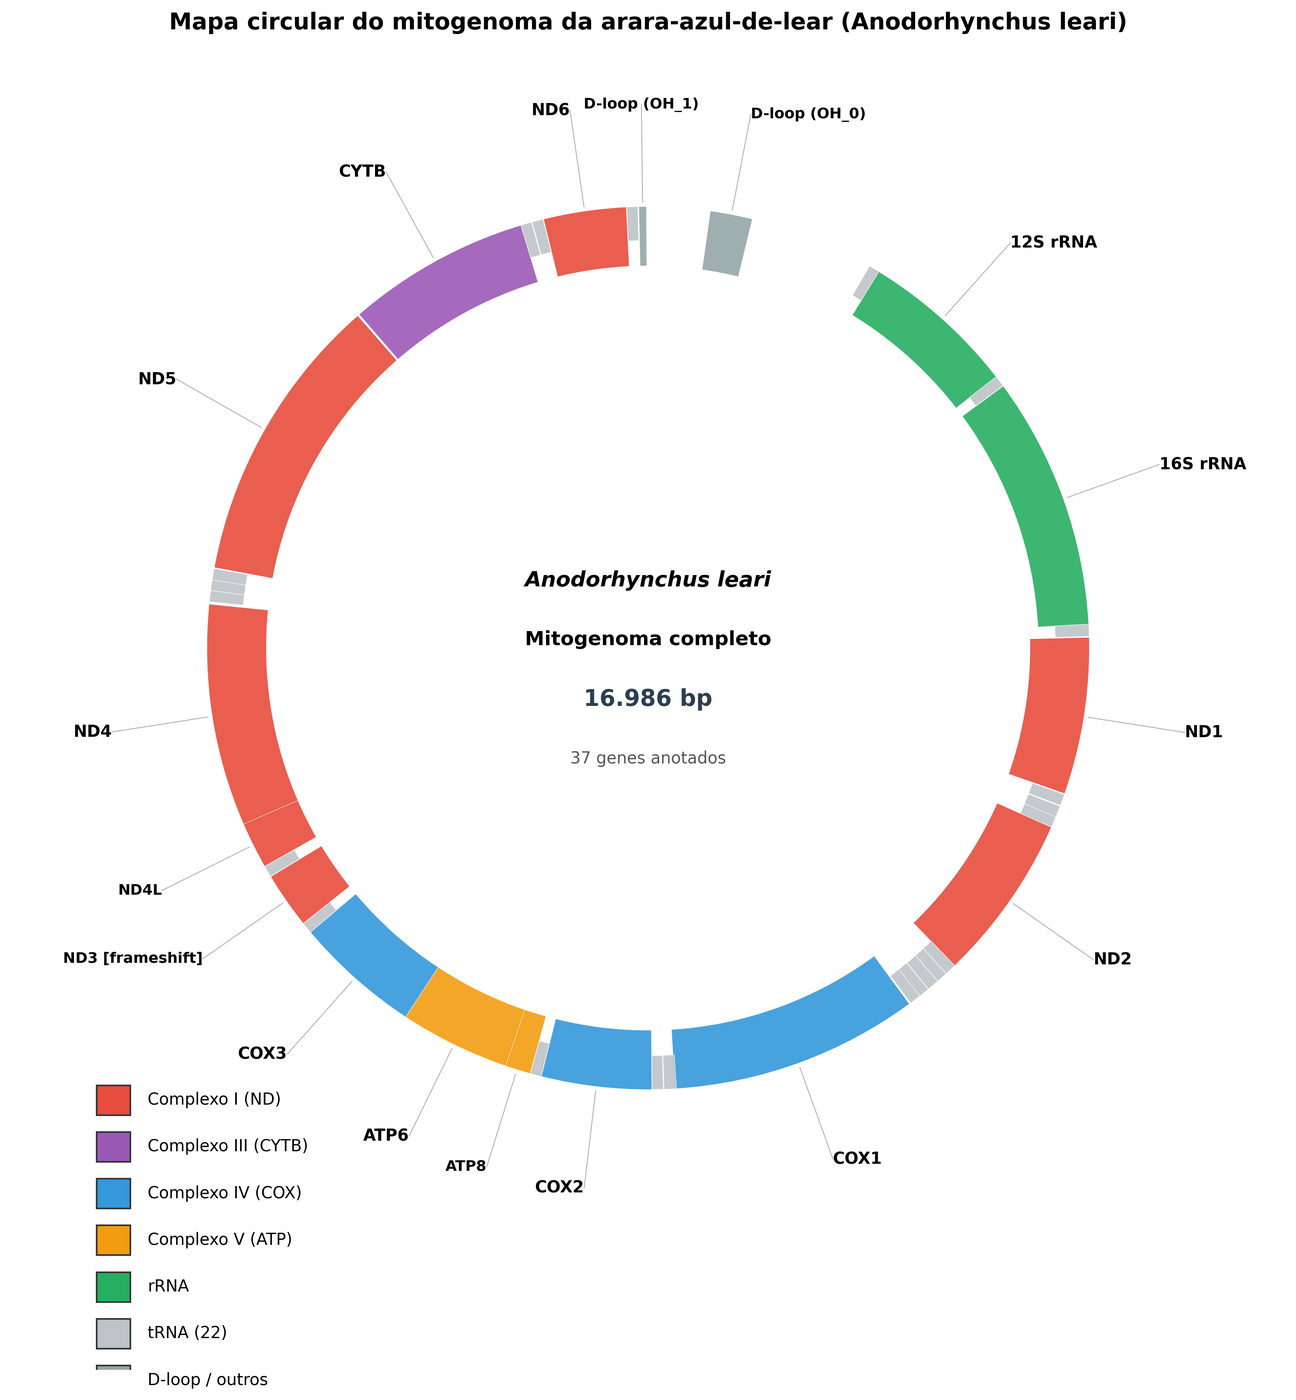
\includegraphics[width=0.70\textwidth]{imagens/mapa_circular_mitogenoma.png}
    \caption{Mapa circular do mitogenoma da arara-azul-de-lear (\textit{A.~leari}, 16.986~bp), com a posição dos 37 genes coloridos por categoria funcional. Gerado automaticamente pelo pipeline via Biopython GenomeDiagram.}
    \label{fig:mapa_circular_leari}
\end{figure}

\section{Genes Codificadores de Proteínas}
\label{sec:cds}

O mitogenoma de \textit{A.~leari} codifica 13 genes de proteínas, correspondentes a subunidades de quatro dos cinco complexos da cadeia respiratória mitocondrial:

\begin{itemize}
    \item \textbf{Complexo I} (NADH desidrogenase): ND1, ND2, ND3, ND4, ND4L, ND5, ND6 --- sete subunidades;
    \item \textbf{Complexo III} (citocromo $b$): CYTB --- uma subunidade;
    \item \textbf{Complexo IV} (citocromo $c$ oxidase): COX1, COX2, COX3 --- três subunidades;
    \item \textbf{Complexo V} (ATP sintase): ATP6, ATP8 --- duas subunidades.
\end{itemize}

O Complexo II (succinato desidrogenase) é ausente em todos os genomas mitocondriais de metazoários, sendo codificado exclusivamente pelo genoma nuclear. Dos 13 genes, 12 são codificados na fita pesada (H-strand), enquanto o ND6 é o único gene codificador na fita leve (L-strand) --- padrão universal em mitogenomas aviários.

A Tabela~\ref{tab:codons} apresenta os códons de início e parada, bem como os tamanhos de cada gene codificador.

\begin{table}[H]
\centering
\caption{Códons de início e parada dos genes codificadores de proteínas de \textit{A.~leari}.}
\label{tab:codons}
\begin{tabular}{@{}llrrr@{}}
\toprule
\textbf{Gene} & \textbf{Início} & \textbf{Parada} & \textbf{Tamanho (bp)} & \textbf{Tamanho (aa)} \\
\midrule
ND1  & ATG & TA(+A)  & 974   & 324 \\
ND2  & ATA & TAA     & 1.041 & 347 \\
COX1 & GTG & AGG     & 1.548 & 516 \\
COX2 & ATG & TAA     & 684   & 228 \\
ATP8 & ATG & TAA     & 168   & 56  \\
ATP6 & ATG & TAA     & 684   & 228 \\
COX3 & ATG & T(+AA)  & 784   & 261 \\
ND4L & ATG & TAA     & 297   & 99  \\
ND4  & ATG & T(+AA)  & 1.378 & 459 \\
ND5  & ATA & TAA     & 1.809 & 603 \\
CYTB & ATG & TAA     & 1.140 & 380 \\
ND6  & ATG & TAG     & 513   & 171 \\
ND3  & ATA & GAA     & 349*  & 118* \\
\bottomrule
\end{tabular}
\begin{flushleft}
\small{* Valores referentes ao gene completo incluindo a região de \textit{frameshift} (ver Seção~\ref{subsec:nd3_frameshift}).}
\end{flushleft}
\end{table}

Três padrões são observados nos códons dos genes codificadores:

(i) O códon de início ATG é o mais frequente, utilizado por 9 dos 13 genes. Os códons alternativos ATA (ND2, ND5, ND3) e GTG (COX1) são aceitos no código genético mitocondrial de vertebrados. As mitocôndrias utilizam um código genético ligeiramente diferente do padrão universal: ATA codifica metionina (em vez de isoleucina), TGA codifica triptofano (em vez de parada), e AGA/AGG funcionam como códons de parada (em vez de arginina) \cite{anderson1981,boore1999}. Esse código corresponde à Tabela 2 do NCBI (\textit{Vertebrate Mitochondrial Code}).

(ii) Três genes (ND1, COX3 e ND4) apresentam códons de parada incompletos, terminando em ``TA'' ou ``T''. Esse fenômeno é consequência do processamento do mRNA policistrônico mitocondrial: a clivagem pós-transcricional do transcrito primário, seguida de poliadenilação, completa o códon de parada TAA pela adição de resíduos de adenina na extremidade 3' do mRNA \cite{anderson1981}.

(iii) O gene ND6, único na fita leve, utiliza o códon de parada TAG, distinto do padrão TAA predominante nos demais genes.

\paragraph*{Análise Ka/Ks.}

A razão Ka/Ks (também denominada dN/dS) é a razão entre substituições não sinônimas ($K_a$, que alteram o aminoácido) e substituições sinônimas ($K_s$, silenciosas). Valores de Ka/Ks $< 1$ indicam seleção purificadora (pressão para manter a sequência proteica), Ka/Ks $> 1$ indica seleção positiva (favorecimento de mudanças), e Ka/Ks $= 1$ indica evolução neutra.

Um padrão universal emerge da literatura: todos os 13 genes codificadores mitocondriais apresentam Ka/Ks $< 1$ em \textbf{todos} os táxons analisados --- aves, répteis, peixes, moluscos, insetos, crustáceos e cnidários \cite{zhan2024,guerreiro2025,shi2024,ye2024,kundu2024,alboasud2024,zhou2024,tao2024}. O gene COX1 é consistentemente o mais conservado (Ka/Ks entre 0,02 e 0,07), refletindo as restrições funcionais severas sobre a subunidade catalítica do Complexo IV. Em contraste, o ATP8 é o mais variável (Ka/Ks entre 0,5 e 0,8), compatível com seu pequeno tamanho e menor número de sítios funcionalmente críticos. Em Planorbidae (caramujos), \citeonline{tao2024} reportaram Ka/Ks $> 1$ para ATP8 em alguns gêneros, sugerindo seleção positiva pontual.

Para \textit{A.~leari}, a conservação de COX1 é evidenciada pela alta identidade com \textit{A.~hyacinthinus}. A comparação direta de Ka/Ks entre as duas espécies de \textit{Anodorhynchus} constitui uma perspectiva futura relevante para identificar genes sob pressão seletiva diferencial.

\paragraph*{Uso de Códons (RSCU).}

O \textit{Relative Synonymous Codon Usage} (RSCU) quantifica a preferência entre códons sinônimos para um mesmo aminoácido. Em genomas mitocondriais, há um viés sistemático em favor de códons com adenina ou timina na terceira posição. \citeonline{shi2024} demonstraram que esse viés é direcionado por seleção natural, e não apenas por pressão mutacional. O padrão é menos extremo em vertebrados, porém detectável \cite{kundu2024,guerreiro2025}. A construção de tabelas de RSCU para \textit{A.~leari} constitui uma perspectiva futura que permitirá comparações detalhadas com outros Psittaciformes.

\subsection{O \textit{Frameshift} do ND3: Uma Assinatura Evolutiva Conservada}
\label{subsec:nd3_frameshift}

O gene ND3 apresenta uma característica incomum compartilhada por aves, tartarugas e crocodilianos: um \textit{frameshift} (mudança de quadro de leitura) que divide o gene em dois quadros abertos de leitura (ORFs) sobrepostos.

\paragraph*{Descoberta.}

O \textit{frameshift} do ND3 foi identificado por \citeonline{mindell1998} em 52 espécies de aves e 10 espécies de tartarugas. Após o nucleotídeo 174 a partir do códon de início, uma inserção de um único nucleotídeo desloca o quadro de leitura em +1. Isso divide o gene em dois ORFs: o primeiro codifica 58 aminoácidos (posições 1--174) e o segundo codifica aproximadamente 59 aminoácidos no quadro deslocado. O MITOS2 anotou essa estrutura como \texttt{nad3\_0} (174~bp) e \texttt{nad3\_1} (180~bp) com sobreposição de 5~bp no sítio de deslizamento --- resultado plenamente consistente com a literatura.

\paragraph*{Mecanismo molecular.}

Duas hipóteses explicam como a proteína ND3 funcional é traduzida apesar da mudança de quadro de leitura:

\begin{enumerate}[label=(\roman*)]
    \item \textbf{\textit{Programmed} +1 \textit{ribosomal frameshifting} (+1 PRF)}: o ribossomo desliza um nucleotídeo adiante (+1) no sítio de \textit{frameshift}, continuando a tradução no novo quadro de leitura. Esse mecanismo difere do $-$1 PRF descrito em retrovírus como HIV e RSV \cite{jacks1988}, onde sequências escorregadias (\textit{slippery sequences}) do tipo X\_XXY\_YYH e pseudonós a jusante induzem o deslizamento reverso \cite{brierley1995,atkins2016}. No +1 PRF, a pausa ribossomal ocorre pela escassez de tRNAs raros complementares ao códon no sítio A, favorecendo cineticamente o deslizamento para frente \cite{harger2002}.

    \item \textbf{Edição pós-transcricional do mRNA}: o nucleotídeo extra é removido por edição do mRNA antes da tradução, restaurando o quadro de leitura original. Evidências para esse mecanismo foram obtidas em estudos de cDNA de tartarugas \cite{russell2008}.
\end{enumerate}

Ambos os mecanismos podem coexistir como redundância funcional, garantindo a produção da proteína ND3 funcional.

\begin{figure}[H]
    \centering
    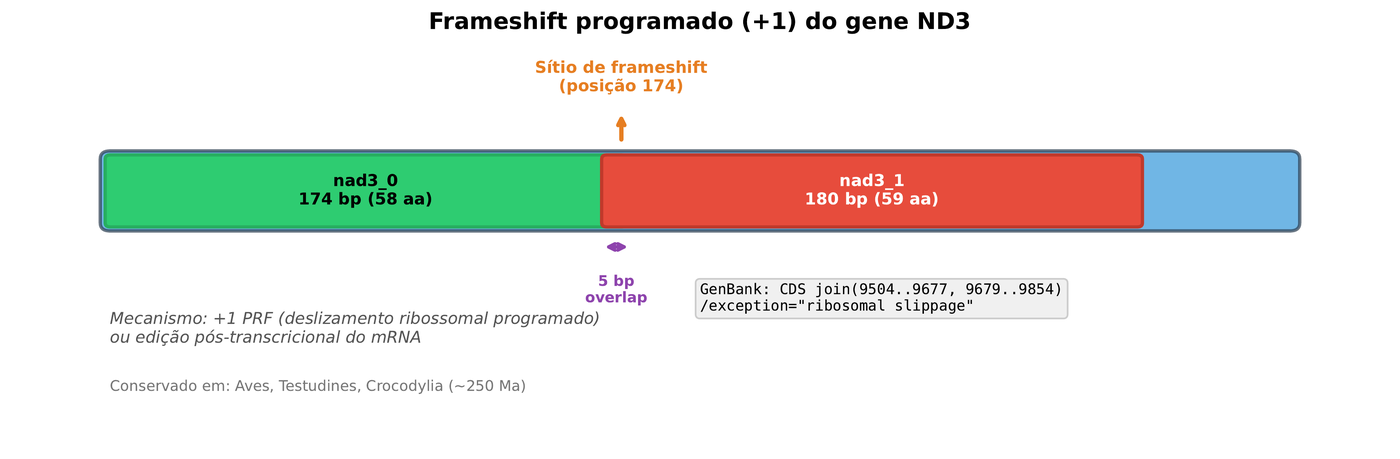
\includegraphics[width=0.85\textwidth]{imagens/frameshift_nd3.png}
    \caption{Diagrama esquemático do \textit{frameshift} do gene ND3: a inserção de um nucleotídeo na posição 174 desloca o quadro de leitura em +1, dividindo o gene em dois ORFs (\texttt{nad3\_0} e \texttt{nad3\_1}).}
    \label{fig:frameshift_nd3}
\end{figure}

\paragraph*{Distribuição taxonômica.}

O \textit{frameshift} do ND3 está presente em todas as aves (Aves), tartarugas (Testudines) e crocodilianos (Crocodylia). \citeonline{russell2008} identificaram inserções de \textit{frameshift} em seis sítios separados em três genes (\textit{nad3}, \textit{nad4l}, \textit{cob}) em tartarugas, e documentaram que \textit{Chelodina parkeri} apresenta reassociação de códon de parada --- o primeiro caso registrado em DNA mitocondrial de vertebrados. O \textit{frameshift} está ausente em mamíferos, anfíbios e na maioria dos peixes. Sua distribuição mapeia o clado Archelosauria (Aves + Crocodylia + Testudines), sugerindo uma única origem há aproximadamente 250 milhões de anos.

\paragraph*{Resultado em \textit{A.~leari}.}

O MITOS2 detectou automaticamente o \textit{frameshift} como \texttt{nad3\_0} + \texttt{nad3\_1}, consistente com a anotação de \textit{A.~hyacinthinus} (NC\_082165.1), onde o ND3 é anotado como:

\begin{lstlisting}
CDS   join(9504..9677,9679..9854)
      /gene="ND3"
\end{lstlisting}

O script \texttt{gff2genbank\allowbreak.py} do pipeline utiliza \texttt{join()} com o qualificador \texttt{/exception=\allowbreak"ribosomal\allowbreak{} slippage"}, conforme as diretrizes do NCBI para submissão ao GenBank.

\section{RNAs Transportadores e Ribossomais}
\label{sec:trna_rrna}

O mitogenoma de \textit{A.~leari} contém 22 genes de tRNA, codificando transportadores para os 20 aminoácidos padrão. Os aminoácidos leucina e serina possuem dois isoaceptores cada: tRNA-Leu(UUR) e tRNA-Leu(CUN); tRNA-Ser(UCN) e tRNA-Ser(AGY). Dos 22 tRNAs, 14 são codificados na fita pesada e 8 na fita leve. A Tabela~\ref{tab:trna} apresenta as características de cada tRNA.

\begin{longtable}{@{}llcl@{}}
\caption{Genes de tRNA do mitogenoma de \textit{A.~leari}.}
\label{tab:trna} \\
\toprule
\textbf{tRNA} & \textbf{Tamanho (bp)} & \textbf{Anticódon} & \textbf{Aminoácido} \\
\midrule
\endfirsthead
\caption[]{Genes de tRNA do mitogenoma de \textit{A.~leari} (continuação).} \\
\toprule
\textbf{tRNA} & \textbf{Tamanho (bp)} & \textbf{Anticódon} & \textbf{Aminoácido} \\
\midrule
\endhead
\bottomrule
\endfoot
tRNA-Phe     & 67 & GAA & Fenilalanina \\
tRNA-Val     & 69 & TAC & Valina \\
tRNA-Leu(UUR) & 74 & TAA & Leucina \\
tRNA-Ile     & 71 & GAT & Isoleucina \\
tRNA-Gln     & 70 & TTG & Glutamina \\
tRNA-Met     & 68 & CAT & Metionina \\
tRNA-Trp     & 70 & TCA & Triptofano \\
tRNA-Ala     & 68 & TGC & Alanina \\
tRNA-Asn     & 73 & GTT & Asparagina \\
tRNA-Cys     & 66 & GCA & Cisteína \\
tRNA-Tyr     & 70 & GTA & Tirosina \\
tRNA-Ser(UCN) & 75 & TGA & Serina \\
tRNA-Asp     & 68 & GTC & Aspartato \\
tRNA-Lys     & 68 & TTT & Lisina \\
tRNA-Gly     & 68 & TCC & Glicina \\
tRNA-Arg     & 69 & TCG & Arginina \\
tRNA-His     & 68 & GTG & Histidina \\
tRNA-Ser(AGY) & 65 & GCT & Serina \\
tRNA-Leu(CUN) & 70 & TAG & Leucina \\
tRNA-Thr     & 67 & TGT & Treonina \\
tRNA-Pro     & 68 & TGG & Prolina \\
tRNA-Glu     & 68 & TTC & Glutamato \\
\end{longtable}

Os tRNAs mitocondriais variam de 65 a 75~bp (média de 69~bp). Todos apresentam a estrutura secundária canônica em trevo (\textit{cloverleaf}), predita por RNAplot/ViennaRNA \cite{lorenz2011} a partir dos modelos de covariância do MITOS2, com uma exceção notável: o tRNA-Ser(AGY) carece do braço DHU, adotando uma conformação simplificada em formato ``D''. Essa ausência é conservada em \textbf{todos} os metazoários há mais de 600 milhões de anos e foi reportada em todos os 15 artigos analisados na revisão de literatura: corais \cite{wei2024}, bivalves \cite{li2023,kartavtsev2024}, estrelas-do-mar \cite{alboasud2024}, afídeos \cite{shi2024}, caramujos planorbídeos \cite{tao2024}, tubarões \cite{ye2024}, raias \cite{guerreiro2025}, lagartos \cite{zhan2024}, anfíbios \cite{hong2024} e teleósteos \cite{kundu2024}. A estrutura simplificada é reconhecida pelo ribossomo mitocondrial por mecanismos alternativos de reconhecimento.

\begin{figure}[H]
    \centering
    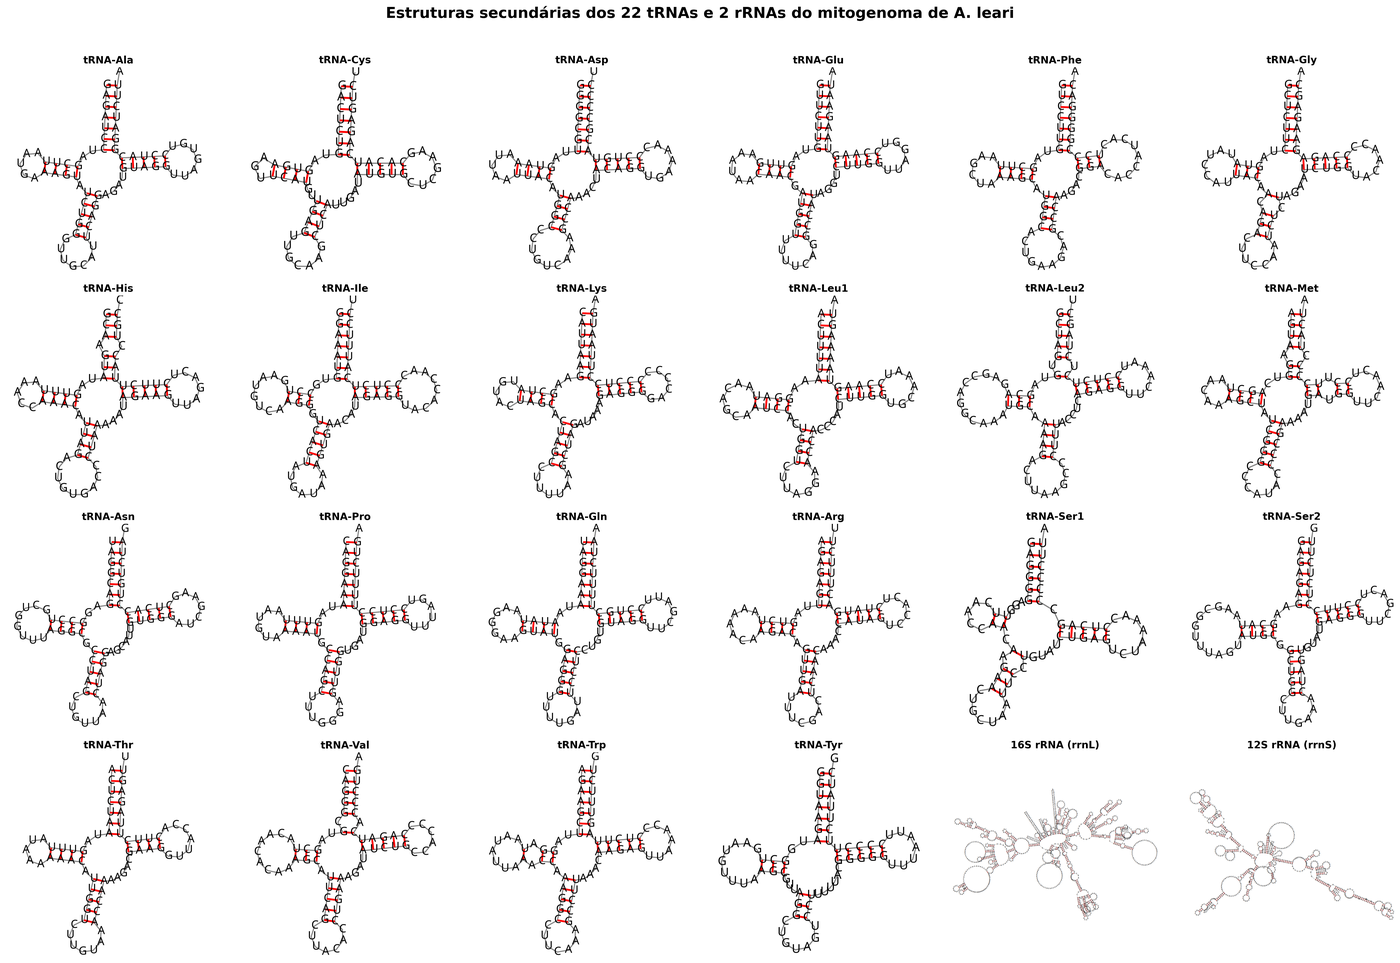
\includegraphics[width=\textwidth]{imagens/painel_trna_rrna.png}
    \caption{Estruturas secundárias em trevo dos 22 tRNAs e 2 rRNAs do mitogenoma de \textit{A.~leari}, preditas pelo MITOS2/RNAplot. O tRNA-Ser(AGY) carece do braço DHU, conformação conservada em todos os metazoários.}
    \label{fig:trna_estruturas}
\end{figure}

O mitogenoma contém dois genes de rRNA: o 12S (rrnS, 970~bp) e o 16S (rrnL, 1.572~bp), localizados entre os genes tRNA-Phe e tRNA-Leu(UUR), separados pelo tRNA-Val. Essa organização é invariável em todos os Psittaciformes. Os ribossomos mitocondriais (mitorribossomos) possuem coeficiente de sedimentação de 55S, com a subunidade menor (28S) contendo o rRNA 12S e a subunidade maior (39S) contendo o rRNA 16S.

\section{Organização Gênica e Comparação com \textit{A.~hyacinthinus}}
\label{sec:organizacao_genica}

A ordem gênica do mitogenoma de \textit{A.~leari} segue o padrão neognata (\textit{standard avian gene order}), descrito por \citeonline{desjardins1990}:

\begin{footnotesize}
\noindent
D-loop --- trnF --- rrnS --- trnV --- rrnL --- trnL2 --- nad1 --- trnI --- trnQ\textsuperscript{(--)} --- trnM --- nad2 --- trnW --- trnA\textsuperscript{(--)} --- trnN\textsuperscript{(--)} --- trnC\textsuperscript{(--)} --- trnY\textsuperscript{(--)} --- cox1 --- trnS2\textsuperscript{(--)} --- trnD --- cox2 --- trnK --- atp8 --- atp6 --- cox3 --- trnG --- nad3 --- trnR --- nad4l --- nad4 --- trnH --- trnS1 --- trnL1 --- nad5 --- cob --- trnT --- trnP\textsuperscript{(--)} --- nad6\textsuperscript{(--)} --- trnE\textsuperscript{(--)} --- D-loop
\end{footnotesize}

\noindent onde o sobrescrito \textsuperscript{(--)} indica genes codificados na fita leve (L-strand).

A comparação direta com o congênere \textit{A.~hyacinthinus} (NC\_082165.1, 16.999~bp) é apresentada na Tabela~\ref{tab:comparacao_hyacinthinus}.

\begin{table}[H]
\centering
\caption{Comparação entre os mitogenomas de \textit{A.~leari} e \textit{A.~hyacinthinus}.}
\label{tab:comparacao_hyacinthinus}
\begin{tabular}{@{}lll@{}}
\toprule
\textbf{Característica} & \textbf{\textit{A.~leari}} & \textbf{\textit{A.~hyacinthinus}} \\
\midrule
Tamanho total   & 16.986 bp & 16.999 bp \\
Diferença       & ---       & $\Delta$ 13 bp \\
CDS             & 13        & 13 \\
tRNAs           & 22        & 22 \\
rRNAs           & 2         & 2 \\
Ordem gênica    & Padrão aviário & Padrão aviário \\
\textit{Frameshift} ND3 & Presente & Presente \\
CDS na fita L   & ND6       & ND6 \\
\bottomrule
\end{tabular}
\end{table}

A diferença de apenas 13~bp ($\sim$0,08\%) entre os dois mitogenomas reflete a divergência recente entre as espécies, consistente com estimativas de separação no Plioceno \cite{tavares2006}. Os mitogenomas são sintênicos --- apresentam a mesma organização estrutural, sem rearranjos detectáveis.

A alta similaridade entre os dois congêneres possui implicações diretas para a conservação. \citeonline{ye2024} demonstraram que o gene COX1 isoladamente é insuficiente para discriminar espécies proximamente relacionadas de tubarões do gênero \textit{Scoliodon}, sendo necessária a análise de múltiplos genes ou do mitogenoma completo. Essa observação é diretamente relevante para \textit{Anodorhynchus}: com apenas 13~bp de divergência total, marcadores conservados como COX1 e CYTB podem ser insuficientes para a discriminação forense entre \textit{A.~leari} e \textit{A.~hyacinthinus}.

\paragraph*{O D-loop como marcador diferencial.}

A região controle (D-loop) apresenta a maior variação inter e intraespecífica no mitogenoma. Em tubarões \textit{Scoliodon}, \citeonline{ye2024} demonstraram a utilidade dessa região para discriminação interespecífica. Em raias \textit{Potamotrygon}, \citeonline{guerreiro2025} identificaram repetições em tandem na região controle, enquanto em afídeos, \citeonline{shi2024} observaram variação geográfica no comprimento do D-loop (650--1.109~bp). A comparação detalhada dos D-loops de \textit{A.~leari} e \textit{A.~hyacinthinus} --- incluindo domínios conservados (\textit{Conserved Central Domains}, CCDs), blocos de sequência conservados (\textit{Conserved Sequence Blocks}, CSBs) e repetições em tandem --- constitui uma perspectiva futura estratégica para a identificação de marcadores forenses diferenciadores entre as duas espécies.

\missingfigure{Diagrama de sintenia comparando mitogenomas de A. leari e A. hyacinthinus}

\section{Implicações para a Conservação}
\label{sec:implicacoes_conservacao}

A disponibilidade do mitogenoma completo de \textit{A.~leari} abre perspectivas concretas para a conservação da espécie, subsidiando aplicações em três frentes complementares: identificação forense, avaliação de diversidade genética e filogeografia.

Antes de discutir essas aplicações, é necessário definir os conceitos fundamentais da genética de conservação empregados nesta análise:

\begin{itemize}
    \item \textbf{Haplótipo}: variante genética definida por mutações específicas, compartilhada por um grupo de indivíduos que a herdou de um ancestral comum. No DNA mitocondrial, cada haplótipo representa uma linhagem materna distinta.

    \item \textbf{Diversidade nucleotídica} ($\pi$): proporção média de nucleotídeos diferentes entre dois indivíduos de uma mesma população. Valores baixos indicam baixa variação genética, típica de populações que sofreram gargalos populacionais.

    \item \textbf{Depressão endogâmica} (\textit{inbreeding depression}): redução da aptidão (\textit{fitness}) decorrente do acúmulo de alelos recessivos deletérios quando indivíduos aparentados se reproduzem --- inevitável em populações pequenas.

    \item \textbf{Filogeografia}: estudo da distribuição geográfica de linhagens genéticas, integrando filogenética molecular e biogeografia.

    \item \textbf{Relógio molecular}: estimativa de tempos de divergência entre espécies com base na taxa de acúmulo de mutações ao longo do tempo.

    \item \textbf{Especiação}: processo pelo qual uma população ancestral se divide em espécies distintas, reprodutivamente isoladas.
\end{itemize}

\paragraph*{Identificação forense.}

O tráfico ilegal de filhotes constitui uma das principais ameaças à arara-azul-de-lear. Um paralelo pode ser traçado com a raia de água doce \textit{Potamotrygon leopoldi} \cite{guerreiro2025}, cujo mitogenoma de 17.504~bp revelou sinais de seleção positiva nos genes ND1, ND4, ND5, COX1 e COX2, associados à adaptação ao ambiente de água doce. O mitogenoma completo viabiliza a criação de marcadores de DNA \textit{barcoding} \cite{hebert2003} para identificação inequívoca da espécie. Os genes COX1 (1.548~bp) e CYTB (1.140~bp) representam a primeira abordagem para laboratórios forenses. Todavia, o COX1 isoladamente é insuficiente para espécies proximamente relacionadas \cite{ye2024}. Modelos de aprendizado de máquina (\textit{Random Forest}, SVM, MLP) com AUC $>$ 0,90, treinados com os 13 genes codificadores, poderiam distinguir \textit{A.~leari} de \textit{A.~hyacinthinus} --- aplicáveis a ovos, penas, tecidos ou indivíduos em cativeiro.

\paragraph*{Avaliação de diversidade genética.}

A população de \textit{A.~leari} sofreu um severo gargalo demográfico entre as décadas de 1970 e 1990, quando foi reduzida a aproximadamente 200 indivíduos \cite{sick1979,icmbio2022}. Gargalos dessa magnitude reduzem drasticamente a variabilidade genética, aumentando a vulnerabilidade a doenças e a depressão endogâmica. A sequência mitocondrial completa permite o sequenciamento da região D-loop de múltiplos indivíduos para estimar o número de haplótipos circulantes, a diversidade nucleotídica ($\pi$) e a estrutura populacional entre os núcleos de Toca Velha e Serra Branca. Esses dados constituem insumos diretos para o Plano de Ação Nacional \cite{icmbio2022} e para decisões de manejo, como translocações entre populações e programas de reprodução em cativeiro.

\paragraph*{Filogeografia e evolução do gênero.}

O mitogenoma completo possibilita análises filogenéticas multigênicas robustas dentro de Psittaciformes. A divergência de 13~bp em relação a \textit{A.~hyacinthinus} pode ser utilizada para calibrar relógios moleculares e estimar tempos de divergência, contribuindo para a compreensão da biogeografia histórica do gênero \textit{Anodorhynchus} e dos processos de especiação na Caatinga \cite{tavares2006}.

\section{Disponibilidade dos Dados}
\label{sec:disponibilidade}

Os dados gerados neste trabalho estão disponíveis nos seguintes formatos:

\begin{itemize}
    \item \textbf{GenBank Flat File} (\texttt{A\_leari.gbk}): formato padrão do NCBI, pronto para submissão. Contém todos os 37 genes anotados, com \texttt{join()} e \texttt{/exception="ribosomal slippage"} para o \textit{frameshift} do ND3.

    \item \textbf{Feature Table} (\texttt{A\_leari.tbl}) e \textbf{FASTA formatado} (\texttt{A\_leari.fsa}): para processamento pela ferramenta \texttt{table2asn} do NCBI.

    \item \textbf{Repositório GitHub}: todo o código-fonte --- Dockerfiles, módulos Nextflow, scripts de análise e configurações de perfil --- está disponível publicamente para reprodutibilidade completa \cite{wilkinson2016}.
\end{itemize}

A disponibilidade pública contribui para a democratização do acesso à bioinformática, permitindo que outros grupos de pesquisa reproduzam as análises ou apliquem o pipeline a outras espécies --- aves, peixes, invertebrados ou qualquer metazoário --- necessitando apenas de um acesso SRA e uma sequência-semente de gene mitocondrial. A generalização do pipeline foi verificada pela execução bem-sucedida em dois táxons distintos (Psittaciformes e Perciformes), reforçando a aderência aos princípios FAIR (\textit{Findable, Accessible, Interoperable, and Reusable}).
